\documentclass[11pt, oneside]{article}   	% use "amsart" instead of "article" for AMSLaTeX format
\usepackage{geometry}                		% See geometry.pdf to learn the layout options. There are lots.
\geometry{letterpaper}                   		% ... or a4paper or a5paper or ... 
%\geometry{landscape}                		% Activate for for rotated page geometry
%\usepackage[parfill]{parskip}    		% Activate to begin paragraphs with an empty line rather than an indent
\usepackage{graphicx}				% Use pdf, png, jpg, or eps§ with pdflatex; use eps in DVI mode
								% TeX will automatically convert eps --> pdf in pdflatex		
\usepackage{amssymb}
\usepackage{amsmath}

\title{Double Integrals - Introduction}
%\author{The Author}
\date{}							% Activate to display a given date or no date

\graphicspath{{/Users/telliott_admin/Dropbox/Tex/png/}}

\begin{document}

\maketitle
%\section{}
% \subsection*{R code}
% \begin{lstlisting}  \end{lstlisting}
% \begin{center} 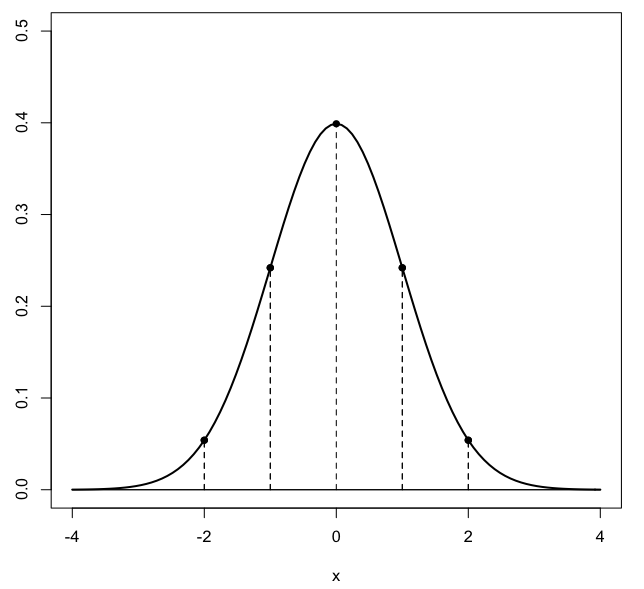
\includegraphics [scale=0.4] {gauss3.png} \end{center}
% \begin{bmatrix} a  &  b \\ c  &  d \end{bmatrix}
% \bigg |_

\large
\noindent

Double integrals start with a function of two variables, say $x$ and $y$, $f(x,y)$.  Think of this as a surface with height $z=f(x,y)$, it could be a sloping roof or something more irregular, but still smooth.  Then the integration is performed over a region (an area) in the xy-plane that is the shadow of the surface.  The double integral is the volume contained between the plane and the surface at $z$, within the bounds of the region $R$.
\[ \int \int_R f(x,y) \ dA = ? \]

As our first example, consider the region to be a rectangle with opposing corners at coordinates $(0,0)$ and $(2,1)$.  

\begin{center} 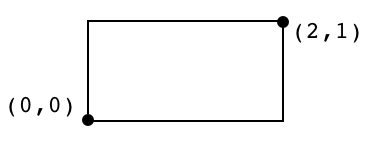
\includegraphics [scale=0.5] {dint1.png} \end{center}

The idea of the integral is that if we slice the volume vertically, say with slices perpendicular to the $x$ axis, we have a standard integral to yield the area of the slice when integrating over $dy$ parallel to the slice, and then in a second integral we add up all of these area slices in the second integral over $x$.  This is known as an \emph{iterated integral}.
\[ \int \int_R f(x,y) \ dA = \int_y \int_x f(x,y) \ dx \ dy = = \int_x \int_y f(x,y) \ dy \ dx = ? \]
Suppose
\[ f(x,y) = xy^2 \]
\[ \int \int_R xy^2 \ dA = ? \]
In this example we sidestep one of the important complications of double integrals compared to single integrals.  Because the area is a rectangle, the bounds of $x$ and $y$ don't depend on where we are in the box, they are the same for each slice.  So, for slices in the vertical direction (integrating over $dy$ first and $dx$ second), we have
\[ \int_{x=0}^{x=2} \int_{y=0}^{y=1} xy^2 \ dy \ dx \]
Here, the \emph{inner} integral is the one we will do first, it is
\[ \int_{y=0}^{y=1} xy^2 \ dy \]
As usual for multivariable calculus, in this computation we treat one variable, here $x$, as a constant.  So we have
\[ \int_{y=0}^{y=1} xy^2 \ dy = \frac{1}{3} xy^3 \ \bigg |_0^1 = \frac{1}{3}x \]
We plug this result into the outer integral
\[ \int_{x=0}^{x=2} \frac{1}{3}x  \ dx = \frac{1}{6} x^2 \ \bigg |_0^2 = \frac{2}{3} \]
Sometimes we will only be able to do a double integral one way, but here we can do it the other way to check
\[ \int_{y=0}^{y=1} \int_{x=0}^{x=2} xy^2 \ dx \ dy \]
Now, the inner integral is 
\[ \int_{x=0}^{x=2} xy^2 \ dx = \frac{1}{2} x^2y^2 \ \bigg |_0^2 = 2y^2 \]
and the outer integral is
\[ \int_{y=0}^{y=1} 2y^2 \ dy = \frac{2}{3}y^3 \ \bigg |_0^1 = \frac{2}{3} \]
They are the same, so that looks good.

Let's do a second example.  Suppose we have the surface $f(x,y) = x^2 + y^2$,  a paraboloid surface opening up.  Our region R is the \emph{Cartesian product} 
\[ R = [-1,1] \times [0,1] \]
We have 
\[ \int \int x^2 + y^2 \ dx \ dy \]
We can do this in either order, so we'll do the inner integral as
\[ \int_{-1}^1 x^2 + y^2 dx = \frac{1}{3}x^3 + xy^2 \ \bigg |_{-1}^{1} = \frac{1}{3} + y^2 - (-\frac{1}{3} - y^2) = \frac{2}{3} + 2y^2 \]
Now the outer integral is
\[ \int_0^1 \frac{2}{3} + 2y^2 \ dy = \frac{2}{3}y + \frac{2}{3}y^3  \ \bigg |_{0}^{1} = \frac{2}{3} + \frac{2}{3} = \frac{4}{3} \]

\subsection*{changed bounds}

\begin{center} 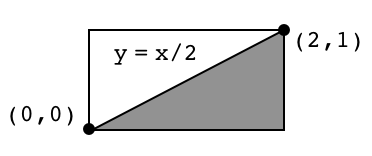
\includegraphics [scale=0.5] {dint2.png} \end{center}

In our second example, we use half of the rectangle, the half that lies below the line $y=x/2$.  Now the upper bound, (the value of $y$) at the top of each slice, is different.

\begin{center} 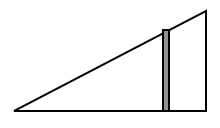
\includegraphics [scale=0.5] {dint3.png} \end{center}

When we integrate $dy$ first, the integral goes from $y=0 \to y=x/2$
\[ \int_{x=0}^{x=2} \int_{y=0}^{y=x/2} xy^2 \ dy \ dx \]
The inner integral is
\[ \int_{y=0}^{y=x/2} xy^2 \ dy = \frac{1}{3} xy^3 \ \bigg |_{y=0}^{y=x/2} = \frac{1}{3}x(\frac{x}{2})^3 = \frac{1}{3} \ \frac{1}{8} \ x^4 \]
and the outer integral is 
\[ \int_{x=0}^{x=2} \frac{1}{3} \ \frac{1}{8}  x^4 \ dx = \frac{1}{3} \ \frac{1}{8}  \frac{x^5}{5} \ \bigg |_{x=0}^{x=2} = = \frac{1}{3} \ \frac{1}{5} \ 4 = \frac{4}{15} \]

On the other hand, if we integrate $dx$ first then the bounds for $x$ are from $x=2y \to x=2$ and $y$ covers the entire range from $y=0 \to 1$. 
\begin{center} 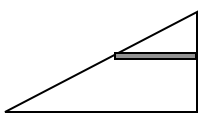
\includegraphics [scale=0.5] {dint4.png} \end{center}

 So we have
\[ \int_{y=0}^{y=1} \int_{x=2y}^{x=2} xy^2 \ dx \ dy \]
The inner integral is
\[ \int_{x=2y}^{x=2} xy^2 \ dy = \frac{1}{2}x^2y^2 \ \bigg |_{x=2y}^{x=2} = 2y^2 - 2y^4 \]
and the outer integral is
\[ \int_{y=0}^{y=1} 2y^2 - 2y^4 \ dy= \frac{2}{3}y^3 - \frac{2}{5}y^5 \ \bigg |_{y=0}^{y=1}  =  \frac{2}{3} - \frac{2}{5} =   \frac{10}{15} - \frac{6}{15} = \frac{4}{15}  \]

\subsection*{Strange limits}
Suppose we do a really simple function with a region whose boundary is something like $y = \ln x$.  We are interested in the region above the curve $y = \ln x$ and below $y=1$.  We go from $x=1$ (where $y=0$) to $x=e$ (where $y=1$).

\begin{center} 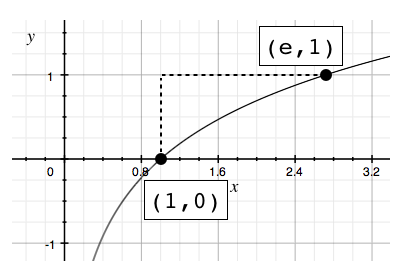
\includegraphics [scale=0.5] {dint5.png} \end{center}

Our simple function is just $1$.  When integrated over the region, this gives the area.
\[ \int \int_R 1 \ dA = A \]
If we integrate $dy$ first, our slices are vertical.  The limits for $y$ are $y = \ln x \to y = 1$.  The limits for $x$ are $x=1 \to x=e$.
\[ \int_{x=1}^{x=e} \int_{y=\ln x}^{y=1} dy \ dx \]
The inner integral is
\[ y  \ \bigg |_{y=\ln x}^{y=1} = 1 - \ln x \]
and the outer integral is
\[ \int_{x=1}^{x=e} 1 - \ln x \ dx =  x - (x \ln x - x) = 2x - x \ \ln x \ \bigg |_{x=1}^{x=e} = 2e - e - 2 + 0 = e - 2 \]

If we do the integral with $dx$ first, we have
\[ \int_{y = 0}^{y=1} \int_{x=1}^{x=e^y} dx \ dy \]
The inner integral is
\[ \int_{x=1}^{x=e^y} dx = x \ \bigg |_{x=1}^{x=e^y} = e^y - 1  \]
and the outer integral is
\[ \int_{y=0}^{y=1}  e^y - 1  \ dy  = e^y - y \ \bigg |_0^1 = e - 1 - 1 + 0 = e - 2 \]

\subsection*{Only one way}
Next, consider
\[ \int \int_R e^{y^2} \ dA \]
We don't have a way to do $dy$ first
\[ \int  e^{y^2} \ dy = ? \]
However
\[ \int  e^{y^2} \ dx = e^{y^2} \ x \]
Now with just the right limits, we might have $x = 0 \to x=y$, then
\[ \int_{x=0}^{x=y}  e^{y^2} \ dx = e^{y^2} \ x \ \bigg |_{x=0}^{x=y} = e^{y^2} \ y \]
We have the $y$ that we need and the outer integral is
\[ \int_{y=0}^{y=1}  e^{y^2} y \ dy = \frac{1}{2} e^{y^2} \ \bigg |_{y=0}^{y=1} = \frac{1}{2}(e-1) \]
\subsection*{Auroux}
In his introduction to double integrals describes the problem of finding the volume under the surface
\[ z = 1 - x^2 - y^2 \]
Visualizing surfaces can be difficult, but here, just set $x=0$ or $y=0$ (separately), then you see that we have a parabola.  This solid is a paraboloid, opening downward, with its apex at $(0,0,1)$.

\begin{center} 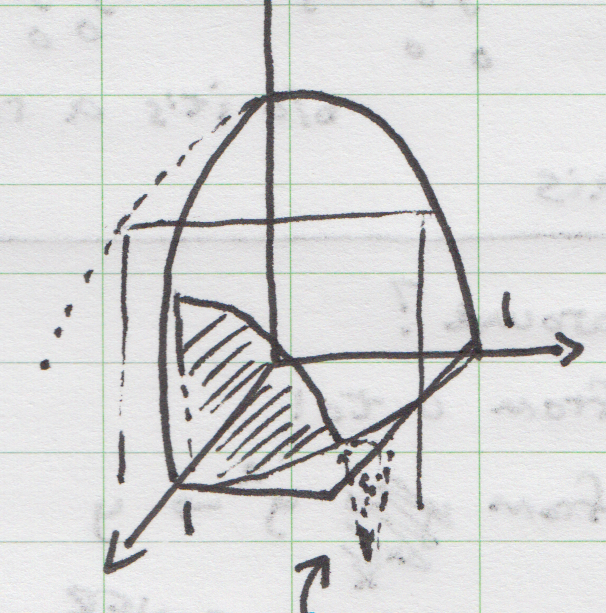
\includegraphics [scale=1.0] {dint.png} \end{center}

The first attempt integrates over the square region $x=0 \rightarrow x=1$ and $y=0 \rightarrow y=1$.  As he points out, this is a bit misguided, because for part of this region, the paraboloid is below the $x,y$-axis.  (If $x=y$ and $z=0$, $x = 1/\sqrt{2}$.  Nevertheless,

\[ \int_0^1 \int_0^1 1 - x^2 - y^2 \ dy \ dx \]
the inner integral is 
\[ y - x^2 y - \frac{1}{3}y^3  \ \bigg |_{0}^{1} = \frac{2}{3} - x^2 \]
and the outer one is
\[  \int_0^1 \frac{2}{3} - x^2 \ dx \]
\[ = \frac{2}{3} x - \frac{1}{3}x^3  \ \bigg |_{0}^{1} = \frac{1}{3} \]

The way to do this problem and actually obtain the volume of the quarter paraboloid is to set up the bounds of integration properly, over the quarter disk.  We can still have $x=0 \rightarrow x=1$ in the outer integral, but for the inner one we use $y=0 \rightarrow y=\sqrt{1-x^2}$.  The changed upper bound makes all the difference.  Now, we have

\[ \int_0^1 \int_0^{\sqrt{1-x^2}} 1 - x^2 - y^2 \ dy \ dx \]
the inner integral is 
\[ (1 - x^2) y - \frac{1}{3}y^3  \ \bigg |_{0}^{\sqrt{1-x^2}} \]
\[= (1-x^2) \sqrt{1-x^2} - \frac{1}{3} (1-x^2)^{3/2} \]
\[ = \frac{2}{3} (1-x^2)^{3/2} \]
Switch to polar coordinates for the outer part

\[ x = \sin \theta \]
\[ dx = \cos \theta \ d \theta \]
\[ \sqrt{1-x^2} = \cos \theta \]
we have
\[ = \frac{2}{3} \int \cos^3 \theta  \cos \theta \ d \theta \]
look it up
\[ = \frac{2}{3} \ [ \ \frac{\cos^3 \theta \ \sin \theta}{3} + \frac{3}{4}( \frac{\theta}{2} + \frac{1}{2} \sin \theta \ \cos \theta ) \ ]  \ \bigg |_{0}^{\pi/2}  \]
At the upper bound, $\cos \pi/2 = 0$ so we get
\[ \frac{2}{3} \ \frac{3}{4} \ \frac{1}{2} \ \frac{\pi}{2} \]
and at the lower bound, $\sin 0 = 0, \theta=0$ so we get $0$.  The result is $\pi/8$.

I would just like to point out another way to find this volume, as a solid of revolution.  Turn the paraboloid and put its apex at the origin, opening to the right.  The equation of its intersection with the $x,y$-plane is just $y=\sqrt{x}$.  For each value of $x=0 \rightarrow x=1$, the cross-section of the paraboloid is a circle of radius $y$ and area $\pi y^2 = \pi x$.  Integrate over the range of $x$

\[ \int_0^1 \pi x \ dx = \pi \frac{1}{2}x^2 = \pi / 2 \]

Recall that we only want $1/4$ of that, or $\pi / 8$.

\subsection*{Two curves}
In Auroux's second example, we have the line $y=x$ and the curve $x=y^2$.  These two curves cross at $(0,0)$ and $(1,1)$, with the line below the curve between these two endpoints.

\begin{center} 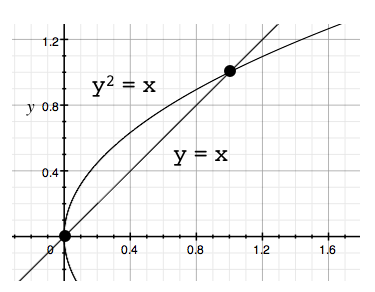
\includegraphics [scale=0.5] {dint6.png} \end{center}

If we integrate $dx$ first, the limits will be $x=y^2 \to x=y$, while if we integrate $dy$ first the limits are $y=x \to y=\sqrt{x}$.

Let's do the area function again ($f(x,y)=1$).
\[ \int \int_R 1 \ dA = ?\]
Start with $dx$ first
\[ \int_{y=0}^{y=1} \int_{x=y^2}^{x=y} \ dx \ dy\]
The inner integral is just
\[ \int_{x=y^2}^{x=y} \ dx  = x  \ \bigg |_{x=y^2}^{x=y} = y - y^2 \]
so the outer integral is
\[ \int_{y=0}^{y=1} y - y^2 \ dy = \frac{1}{2}y^2 - \frac{1}{3}y^3 \ \bigg |_{y=0}^{y=1} =  \frac{1}{2} - \frac{1}{3} = \frac{1}{6} \]
Doing it the other way
\[ \int_{x=0}^{x=1} \int_{y=x}^{y=\sqrt{x}} \ dy \ dx\]
The inner integral is
\[ \int_{y=x}^{y=\sqrt{x}} \ dy  = y  \ \bigg |_{y=x}^{y=\sqrt{x}} = \sqrt{x} - x \]
so the outer integral is
\[ \int_{x=0}^{x=1}\sqrt{x} - x \ dx = \frac{2}{3} x^{3/2} - \frac{1}{2}x^2  \ \bigg |_{x=0}^{x=1} = \frac{2}{3} - \frac{1}{2} = \frac{1}{6} \]

\subsection*{Circle}
Consider a circle of radius $a$ centered at the origin.
\[ x^2 + y^2 = a^2 \]
\[ y = \sqrt{a^2-x^2} \]
This problem is symmetrical so we will only do it one way, integrating over $dy$ first.  
\begin{center} 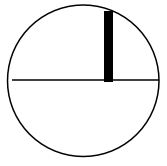
\includegraphics [scale=0.5] {dint7.png} \end{center}

Again, we will do the area function, and we will do only the first quadrant
\[ \int_{x=0}^{x=a}  \int_{y=0}^{y=\sqrt{a^2-x^2}} \ dy \ dx \]
The inner integral is just
\[ \int_{y=0}^{y=\sqrt{a^2-x^2}} \ dy = \sqrt{a^2-x^2} \] 
so now we have for the outer integral
\[ \int_{x=0}^{x=a}  \sqrt{a^2-x^2} \ dx \]
Substitute
\[ x = a \sin \theta, \ \ dx = a \cos \theta \ d \theta \]
For the limits we will have, when $x = 0 \to \theta = 0$ and when $x=a \to \theta=\pi/2$.  (Note that this substitution doesn't match the figure above, so the limits are a bit different.  We used $x=a \sin \theta$).

\[ \int_{x=0}^{x=a}  \sqrt{a^2-x^2} \ dx = \int_{\theta=0}^{\theta=\pi/2} \sqrt{a^2-a^2sin^2\theta} \ a \ cos\ \theta \ d \theta =  a^2 \int_{\theta=0}^{\theta=\pi/2} cos^2\theta \ d \theta \]
\[ = \frac{a^2}{2} \ [ \theta + \sin \ \theta \cos \ \theta \ ] \ \bigg |_{\theta=0}^{\theta=\pi/2} = \frac{a^2}{2} \frac{\pi}{2} =  \frac{\pi}{4} a^2 \] 

\subsection*{Paul}
Here are a couple of examples from Paul's online notes.  The first one is over the region defined by 
\[ R = [-1,2] \times [0,1] \]
What this means is that $x = -1 \to 2$ and y = $0 \to 1$.  The integral is
\[ \int \int_R xe^{xy} \ dA \]
We can see that this will be better to do with $dy$ first.  To make it crystal clear, let's substitute 
\[ u = xy, \ \ du = x \ dy \]
\[ \int xe^{xy} \ dy = \int e^u \ du = e^u = e^{xy} \ \bigg |_0^1 =  e^x - 1 \]
and the outer integral is
\[ \int_{-1}^2 e^x - 1 \ dx = e^x - x  \ \bigg |_{-1}^2 = e^2 - 2 - e^{-1} + 1 = e^2 - e^{-1} - 1 \]

In the next one, we are given the integral already set up
\[ \int_{x=0}^{x=3} \int_{y=x^2}^{y=9} x^3 e^{y^3} \ dy \ dx \]
And of course the problem is that we can't do it this way.  We can do it with $dx$ first, but we need to understand the region that we are integrating over. 

If you draw a sketch, you will see that it is the region above $y=x^2$ and below $y=9$.  We are adding up the slices $f(x,y)$ for $y=x^2 \to y=9$ for every $x = 0 \to 3$.

So our new limits (for slices of the area parallel to the x-axis), we add up $f(x,y)$ for $x=0 \to x=\sqrt{y}$ for every $y = 0 \to 9$.

\[ \int_{0}^9 \int_0^{\sqrt{y}} x^3 e^{y^3} \ dx \ dy \]

So the inner integral is
\[ \int_0^{\sqrt{y}} x^3 e^{y^3} \ dx = \frac{1}{4}x^4 e^{y^3} \ \bigg |_{0}^{\sqrt{y}} = \frac{1}{4}y^2 e^{y^3} \]
Now let 
\[ u = y^3, \ \ du = 3y^2 \ dy, \ \ \frac{1}{3} du = y^2 \ dy \]
and the outer integral is
\[ \int_{0}^9 \frac{1}{4}y^2 e^{y^3} \ dy = \frac{1}{4} \ \frac{1}{3} e^u \ du = \frac{1}{12} e^u = \frac{1}{12} e^{y^3}   \ \bigg |_{0}^9 = \frac{1}{12} (e^{9^3} - 1)\]

Finally, let's recall that in single-variable calculus, to obtain the area between two curves ($g_1(x)$ and $g_2(x)$) for $x = a \to b$ we would integrate the two separately and subtract the lower from the upper.
\vspace{2 mm}

\noindent where the second is always larger than the first $g_2(x) > g_1(x) \ \forall \ x \in [a,b] $.
\[ A = \int_a^b g_2(x) - g_1(x) dx \]

In multi-variable calculus to get the area we integrate

\[ \int \int_R dA \]
over the appropriate bounds.  Here, that leads to
\Large
\[ \int_{x=a}^{x=b} \int_{y=g_1(x)}^{y=g_2(x)} \ dy \ dx = \int_{x=a}^{x=b} g_2(x) - g_1(x) \ dx \]
\large
which is exactly the same thing.


\end{document}  